\documentclass[border=0.2cm]{standalone}
\usepackage{amsmath}
\usepackage{tikz}
\usetikzlibrary{arrows}
\usetikzlibrary{automata, arrows.meta, positioning}
\usepackage{pgfplots}

\begin{document}
    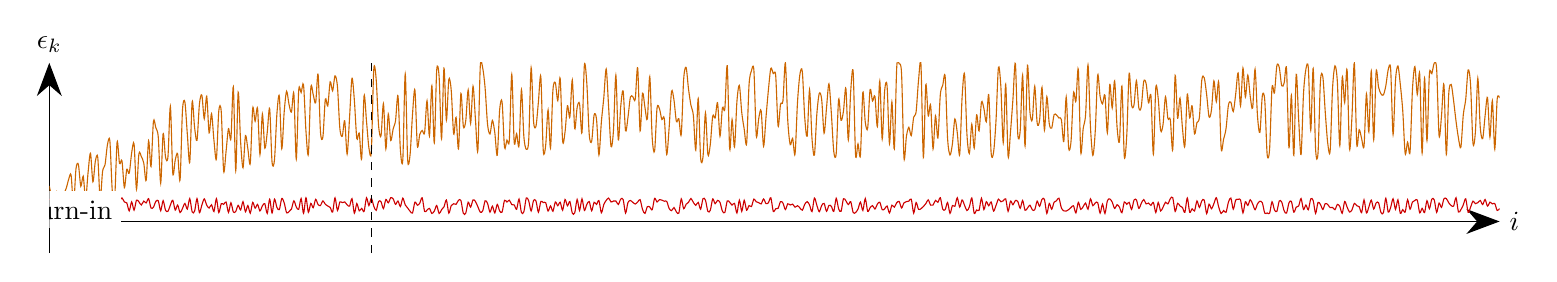
\begin{tikzpicture}[samples=600, domain=0:5*360]
        \begin{axis}[
            width=20cm, height=4cm,
            enlarge x limits=false,
            enlarge y limits=false,
            xtick=\empty, ytick=\empty,
            axis lines*=middle,
            x axis line style = {-{Stealth[scale=2.5]}},
            y axis line style = {-{Stealth[scale=2.5]}},
            axis lines* = middle, xlabel={$i$}, ylabel={$\epsilon_k$},
            every axis y label/.style={at=(current axis.above origin),anchor=south},
            every axis x label/.style={at=(current axis.right of origin),anchor=west},
        ]
        
        \addplot [no markers, smooth, color=orange!80!black] {12/(1+exp(-x/100))-5+rand*3/(1+exp(-x/100))};
        \addplot [no markers, smooth, color=red!80!black] {1+rand*0.5};
        \addplot [dashed, mark=none] coordinates {(400, -2) (400, 10)};  
        \draw [yshift=0.15cm, latex-latex](40, 0) -- node [fill=white] {Burn-in} (0, 0);        
                \end{axis}  
    \end{tikzpicture}
\end{document}